\section{Nulkliner}
Dette afsnit er baseret på \citep[afsnit 9.1]{Hirsch} \\
Når vi skal analysere et ikke-lineært system, som Lotka-Volterra modellen, er bestemmelsen af nulkliner et nyttigt redskab.

\begin{definition}[Nulkliner]\label{NulKliner}
Lad 
\\
$$\dot{y}(t) = \frac{d\vec{y}}{dt} = 
\begin{bmatrix}
\frac{dy_1}{dt} \\
\frac{dy_2}{dt}\\
\vdots \\
\frac{dy_n}{dt}
\end{bmatrix}
=
\begin{bmatrix}
f_1(t, y_1(t), y_2(t), \hdots, y_n(t))\\
f_2(t, y_1(t), y_2(t), \hdots, y_n(t))\\
\vdots \\
f_n(t, y_1(t), y_2(t), \hdots, y_n(t))
\end{bmatrix}$$
\\
være et differentialligningssystem. \\
$y_j$-nulklinen er mængden af punkter, hvor $\frac{dy_j}{dt}=0$ 
\end{definition}
Det ses, at de steder, hvor alle nulklinerne skærer hinanden, er systemets ligevægtspunkter. \\
Har man fundet alle nulklinerne for et system i $\mathbb{R}^n$, deler disse nulkliner sædvanligvis $\mathbb{R}^n$ op i regioner, hvor $y_j$-komponenterne i vektorfeltet peger i enten positiv eller negativ retning. \\
Ser vi på et førsteordens differentialligningssystem bestående af to funktioner, kan vi nemmere illustrere nulklinernes anvendelse.
\begin{Example}\textnormal{Fra \citep[s. 191]{Hirsch}}\\
\textnormal{Givet differentialligningssystemet:}
\begin{align*}
    x'(t)&=y(t)-x(t)^2 \\
    y'(t)&=x(t)-2
\end{align*}
\textnormal{$x$-nulklinen er parablen $y(t)=x(t)^2$, og $y$-nulklinen er den vertikale linje $x=2$. De to nulkliner skærer hinanden i punktet $(2,4)$. Nulklinerne deler $\mathbb{R}^2$ op i 4 regioner $A,B,C,D$, som vist i figur \ref{nulkliner}. Når først vi har fået delt $\mathbb{R}^2$ op i regioner, kan vektorfeltets generelle retning, i hver af disse regioner, bestemmes. Dette gøres ved at vælge et tilfældigt punkt i hver region og udregne vektorfeltets retning i dette punkt. Da det kun er på nulklinerne, at vektorfeltet er parallelt med enten første- eller andenaksen, vil vinklerne for alle vektorer i hver region tilhøre et bestemt af følgende åbne intervaller: $]0,-\frac{\pi}{2}[, \ ]\frac{\pi}{2},\pi[,\ ]\pi,-\frac{\pi}{2}[,\ ]-\frac{\pi}{2},0[$. Punktet $(1,2)$ ligger i region A i figur \ref{nulkliner}(a). I dette punkt har vektorfeltet retningen $(1,-2)$, hvilket betyder, at vinklerne for alle vektorerne i denne region ligger i intervallet $]-\frac{\pi}{2},0[$.}

\begin{figure} [H]
    \centering
    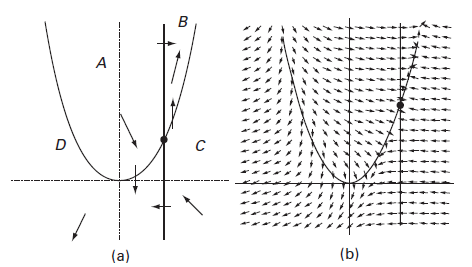
\includegraphics[scale=0.8]{Images/nulkliner.png}
    \caption{Nulklinerne og vektorfeltet for systemet. Figuren er taget fra \citep[s. 191]{Hirsch}}
    \label{nulkliner}
\end{figure}
\end{Example}